\documentclass{beamer}
\usetheme{Warsaw}

\usepackage{graphicx} % Allows including images
\usepackage{booktabs} % Allows the use of \toprule, \midrule and \bottomrule in tables
\usepackage{listings}
\usepackage[utf8]{inputenc}
\usepackage[overlay,absolute]{textpos}
\usepackage{tikz}
\usetikzlibrary{arrows}

\AtBeginSection[]
{
\begin{frame}<beamer>
\frametitle{Plan}
\tableofcontents[
  currentsection,
  hideothersubsections
]
\end{frame}
}

\lstset{language=C++,
                basicstyle=\ttfamily,
                keywordstyle=\color{green}\ttfamily,
                stringstyle=\color{red}\ttfamily,
                commentstyle=\color{cyan}\ttfamily,
                morecomment=[l][\color{magenta}]{\#},
                escapechar=@
}

\setbeamercolor{normal text}{fg=white,bg=black!90}
\setbeamercolor{structure}{fg=white}

\setbeamercolor{alerted text}{fg=red!85!black}

\setbeamercolor{item projected}{use=item,fg=black,bg=item.fg!35}

\setbeamercolor*{palette primary}{use=structure,fg=structure.fg}
\setbeamercolor*{palette secondary}{use=structure,fg=structure.fg!95!black}
\setbeamercolor*{palette tertiary}{use=structure,fg=structure.fg!90!black}
\setbeamercolor*{palette quaternary}{use=structure,fg=structure.fg!95!black,bg=black!80}

\setbeamercolor*{framesubtitle}{fg=white}

\setbeamercolor*{block title}{parent=structure,bg=black!60}
\setbeamercolor*{block body}{fg=black,bg=black!10}
\setbeamercolor*{block title alerted}{parent=alerted text,bg=black!15}
\setbeamercolor*{block title example}{parent=example text,bg=black!15}

\author[Félix-Antoine Ouellet]{Félix-Antoine Ouellet}

\title[Lock-free\hspace{2em}\insertframenumber/\inserttotalframenumber]{Programmation parallèle sans verrous}

\institute{Université de Sherbrooke}

\date{16 octobre 2014}

\begin{document}

\begin{frame}
\titlepage % Print the title page as the first slide
\end{frame}

\begin{frame}
\tableofcontents[hideallsubsections]
\end{frame}

\section{Motivation}
\subsection{Programmation parallèle traditionnelle}
\begin{frame}[fragile]
\frametitle{Programmation parallèle traditionnelle}
\framesubtitle{Exemple}
\begin{lstlisting}
void ThreadSafeIntStack::push(int val) {
  std::lock_guard<std::mutex> lock(m_Mutex);
  m_Stack.push(val);
}

int ThreadSafeIntStack::pop() {
  std::lock_guard<std::mutex> lock(m_Mutex);
  m_Stack.pop();
}
\end{lstlisting}
\end{frame}

\subsection{Problèmes}
\begin{frame}
\frametitle{Problèmes}
\begin{itemize}
\item Coût des verrous
\item Inversion de priorités
\end{itemize}
\end{frame}

\section{Définition}
\begin{frame}
\frametitle{Définitions}
Il existe diverses définitions selon le niveau de garanties fourni.
\begin{itemize}
\item Sans attente
\item Sans verrous
\item Sans obstruction
\end{itemize}
\end{frame}

\defverbatim{\Wait}{%
\begin{lstlisting}
void IncrementRefCounter(Object *obj) {
    atomic_increment(obj->rc);
}
\end{lstlisting}}

\subsection{Sans attente}
\begin{frame}[fragile]
\frametitle{Sans attente}
Chaque fil d'exécution s'exécute dans un nombre fini d'étapes sans égard pour des facteurs externes.

\only<2>{
Exemple:
\Wait
}
\end{frame}

\defverbatim{\Lock}{%
\begin{lstlisting}
void StackPush(Stack *s, Node *n) {
  Node* head;
  do {
    head = s->head;
    n->next = head;
  }
  while (!CompareExchange(s->head, head, n));
}
\end{lstlisting}}

\subsection{Sans verrous}
\begin{frame}[fragile]
\frametitle{Sans verrous}
Le système en entier va continuer de progresser malgré que certains fils d'exécution ne progressent pas.

\only<2>{
Exemple:
\Lock
}
\end{frame}

\defverbatim{\Obs}{%
\begin{lstlisting}
?
\end{lstlisting}}

\subsection{Sans obstruction}
\begin{frame}[fragile]
\frametitle{Sans obstruction}
Un fil d'exécution exécuter en isolation va terminer dans un nombre fini d'étapes.

\only<2>{
Exemple:
\Obs
}
\end{frame}

\section{Techniques}
\subsection{Read-Modify-Write}
\begin{frame}
\frametitle{Read-Modify-Write}
\framesubtitle{Haut niveau}
\begin{itemize}
\item Classe d'opérations atomiques
\item Souvent utilisé pour implémenter des mutex
\item Exécute une lecture et une écriture
\end{itemize}
\end{frame}

\begin{frame}
\frametitle{Read-Modify-Write}
\framesubtitle{Opérations}
\begin{itemize}
\item Test-And-Set
\item Fetch-And-Add
\item Compare-And-Swap
\end{itemize}
\end{frame}

\subsection{Compare-And-Swap}
\begin{frame}[fragile]
\frametitle{Compare-And-Swap}
\framesubtitle{Haut niveau}
\begin{lstlisting}
int CompareAndSwap(int *reg, int oldVal,
                   int newVal) {
  int r = *reg;
  if (*reg == oldVal)
      *reg = newVal;
  return r;
}
\end{lstlisting}
\end{frame}

\begin{frame}[fragile]
\frametitle{Compare-And-Swap}
\framesubtitle{Assembleur}
\begin{center}
\Huge CMPXCHG
\end{center}
\end{frame}

\begin{frame}[fragile]
\frametitle{Compare-And-Swap}
\framesubtitle{Pratique}
\begin{lstlisting}
void LockFreeList::PushFront(Node *newHead) {
  for (;;) {
    Node *oldHead = m_Head;
    newHead->next = oldHead;
    if (CompareAndSwap(&m_Head, newHead, 
                       oldHead) == oldHead)
      return;
  }
}
\end{lstlisting}
\end{frame}

\subsection{Problème ABA}
\begin{frame}
\frametitle{Problème ABA}
\framesubtitle{Description sommaire}
Modifications par un fil d'exécution à une structure partagée dont les autres fils d'exécution n'ont pas connaissance.
\end{frame}

\begin{frame}[fragile]
\frametitle{Problème ABA}
\framesubtitle{Exemple - Code}
\begin{lstlisting}
void LockFreeList::PushFront(Node *newHead) {
  for (;;) {
    Node *oldHead = m_Head;
    newHead->next = oldHead;
    if (CompareAndSwap(&m_Head, newHead, 
                       oldHead) == oldHead)
      return;
  }
}
\end{lstlisting}
\end{frame}

\begin{frame}
\frametitle{Problème ABA}
\framesubtitle{Exemple - Exécution}
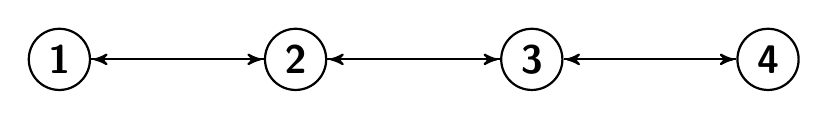
\begin{tikzpicture}[->,>=stealth',shorten >=1pt,auto,node distance=3cm,
  thick,main node/.style={circle,draw,font=\sffamily\Large\bfseries}]

  \node[main node] (1) {1};
  \node[main node] (2) [right of=1] {2};
  \node[main node] (3) [right of=2] {3};
  \node[main node] (4) [right of=3] {4};

  \path[every node/.style={font=\sffamily\small}]
    (1) edge node [right] {} (2)
    (2) edge node [right] {} (3)
        edge node [left] {} (1)
    (3) edge node [right] {} (4)
    	edge node [left] {} (2)
    (4) edge node [left] {} (3);
\end{tikzpicture}
\end{frame}

\begin{frame}
\frametitle{Problème ABA}
\framesubtitle{Exemple - Exécution}
\begin{textblock}{5}(5, 5)
	 Thread 1 \\
	 PushFront();
\end{textblock}
\begin{textblock}{5}(10, 5)
	 \textcolor{gray}{Thread 2} \\
\end{textblock}
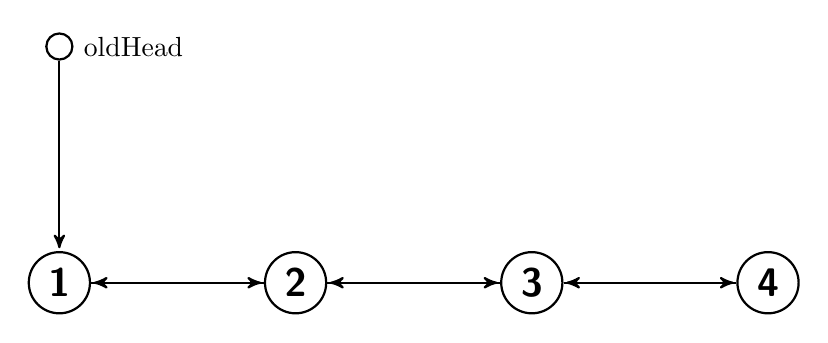
\begin{tikzpicture}[->,>=stealth',shorten >=1pt,auto,node distance=3cm,
  thick,main node/.style={circle,draw,font=\sffamily\Large\bfseries}]

  \node[main node] (1) {1};
  \node[main node] (2) [right of=1] {2};
  \node[main node] (3) [right of=2] {3};
  \node[main node] (4) [right of=3] {4};
  \node[main node, label=right:oldHead] (T1) [above of=1] {};

  \path[every node/.style={font=\sffamily\small}]
    (1) edge node [right] {} (2)
    (2) edge node [right] {} (3)
        edge node [left] {} (1)
    (3) edge node [right] {} (4)
    	edge node [left] {} (2)
    (4) edge node [left] {} (3)
    (T1) edge node [->, thick] {} (1);
\end{tikzpicture}
\end{frame}

\begin{frame}
\frametitle{Problème ABA}
\framesubtitle{Exemple - Exécution}
\begin{textblock}{5}(5, 5)
	 \textcolor{gray}{Thread 1} \\
	 \textcolor{gray}{PushFront();}
\end{textblock}
\begin{textblock}{5}(10, 5)
	 Thread 2 \\
	 PopFront(); \\
\end{textblock}
\begin{tikzpicture}[->,>=stealth',shorten >=1pt,auto,node distance=3cm,
  thick,main node/.style={circle,draw,font=\sffamily\Large\bfseries}]

  \node[main node] (2) [right of=1] {2};
  \node[main node] (3) [right of=2] {3};
  \node[main node] (4) [right of=3] {4};
  \node[main node, label=right:\textcolor{gray}{oldHead}, draw=gray] (T1) [above of=1] {};

  \path[every node/.style={font=\sffamily\small}]
    (2) edge node [right] {} (3)
    (3) edge node [right] {} (4)
    	edge node [left] {} (2)
    (4) edge node [left] {} (3)
    (T1) edge [->, thick, draw=gray] node {} (1);
\end{tikzpicture}
\end{frame}

\begin{frame}
\frametitle{Problème ABA}
\framesubtitle{Exemple - Exécution}
\begin{textblock}{5}(5, 5)
	 \textcolor{gray}{Thread 1} \\
	 \textcolor{gray}{PushFront();}
\end{textblock}
\begin{textblock}{5}(10, 5)
	 Thread 2 \\
	 PopFront(); \\
	 PopFront(); \\
\end{textblock}
\begin{tikzpicture}[->,>=stealth',shorten >=1pt,auto,node distance=3cm,
  thick,main node/.style={circle,draw,font=\sffamily\Large\bfseries}]

  \node[main node] (3) [right of=2] {3};
  \node[main node] (4) [right of=3] {4};
  \node[main node, label=right:\textcolor{gray}{oldHead}, draw=gray] (T1) [above of=1] {};

  \path[every node/.style={font=\sffamily\small}]
    (3) edge node [right] {} (4)
    (4) edge node [left] {} (3)
    (T1) edge [->, thick, draw=gray] node {} (1);
\end{tikzpicture}
\end{frame}

\begin{frame}
\frametitle{Problème ABA}
\framesubtitle{Exemple - Exécution}
\begin{textblock}{5}(5, 5)
	 \textcolor{gray}{Thread 1} \\
	 \textcolor{gray}{PushFront();}
\end{textblock}
\begin{textblock}{5}(10, 5)
	 Thread 2 \\
	 PopFront(); \\
	 PopFront(); \\
	 PushFront(node1);
\end{textblock}
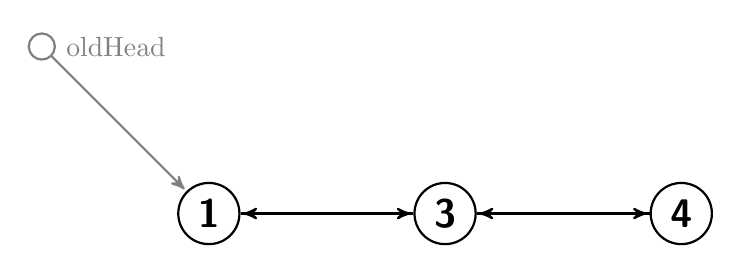
\begin{tikzpicture}[->,>=stealth',shorten >=1pt,auto,node distance=3cm,
  thick,main node/.style={circle,draw,font=\sffamily\Large\bfseries}]

  \node[main node] (1) {1};
  \node[main node] (3) [right of=1] {3};
  \node[main node] (4) [right of=3] {4};
  \node[main node, label=right:\textcolor{gray}{oldHead}, draw=gray] (T1) [above left of=1] {};

  \path[every node/.style={font=\sffamily\small}]
    (1) edge node [right] {} (3)
    (3) edge node [right] {} (4)
    	edge node [left] {} (1)
    (4) edge node [left] {} (3)
    (T1) edge [->, thick, draw=gray] node {} (1);
\end{tikzpicture}
\end{frame}

\section{Modèle mémoire}
\subsection{Modèle mémoire}
\begin{frame}
\frametitle{Modèle mémoire}
\begin{itemize}
\item Existe au niveau du langage et du processeur
\item Décrit l'interaction possible entre fils d'exécution
\begin{itemize}
\item Atomicité
\item Visibilité
\item Ordonnancement
\end{itemize}
\end{itemize}
\end{frame}

\subsection{Visibilité}
\begin{frame}[fragile]
\frametitle{Visibilité}
\framesubtitle{Problème}
\begin{lstlisting}
// Processeur #1
while (f) {
  print x;
}

// Processeur #2
x = 42;
f = false;
\end{lstlisting}
\end{frame}

\begin{frame}[fragile]
\frametitle{Visibilité}
\framesubtitle{Solution}
\begin{lstlisting}
// Processeur #1
while (f);
WriteMemoryBarrier();
print x;

// Processeur #2
x = 42;
WriteMemoryBarrier();
f = false;
\end{lstlisting}
\end{frame}

\subsection{Ordonnancement}
\begin{frame}[fragile]
\frametitle{Ordonnancement}
\framesubtitle{Problème}
\begin{lstlisting}
struct foo {
  int a;
  int b;
};
struct foo *gp = NULL;
/* . . . */
p = kmalloc(sizeof(*p), GFP_KERNEL);
p->a = 1;
p->b = 2;
gp = p;
\end{lstlisting}
\end{frame}

\begin{frame}[fragile]
\frametitle{Ordonnancement}
\framesubtitle{Solution}
\begin{lstlisting}
struct foo {
  int a;
  int b;
};
struct foo *gp = NULL;
/* . . . */
p = kmalloc(sizeof(*p), GFP_KERNEL);
WriteMemoryBarrier();
p->a = 1;
p->b = 2;
gp = p;
WriteMemoryBarrier();
\end{lstlisting}
\end{frame}

\section{Conclusion}
\begin{frame}
\frametitle{Conclusion}
\begin{itemize}
\item On jongle avec des lames de rasoir
\item<2-> Il faut connaître ses outils logiciels et matériels
\end{itemize}
\end{frame}

\end{document}